\large{
Nel capitolo che segue sarà trattata l'analisi e lo studio delle primitive di interazione applicabili ad un grafo clusterizzato. In particolare saranno divise a seconda della tipologia di operazione che si andrà ad eseguire sulla struttura dati o sulla loro visualizzazione mediante l'interazione. Le soluzioni trovate sono applicabili a qualunque grafo clusterizzato e tentano di dare almeno in parte uno standard per ciò che ne concerne la visualizzazione. Le seguenti primitive di interazione sono realizzabili ed eseguibili in qualunque sistema di grado $3$ ovvero in grado di creare e trasformare i dati e la conseguente rappresentazione.
\section{creazione di un oggetto}
Per quanto riguarda le primitive di interazione mediante le quali viene eseguita una operazione di creazione, è possibile creare tre tipologie di elementi definiti nodi, cluster ed archi, con proprietà diverse a seconda della propria rappresentazione. Si ricorda inoltre che la visualizzazione è esclusiva per i dati che sono conosciuti o sono stati importati e non è possibile avere una visualizzazione senza la presenza di un dato. Come sarà visto meglio di seguito è possibile visualizzare i dati in più viste diverse essendo un grafo clusterizzato una composizione di un grafo e di un albero di inclusione.\\
Per la rappresentazione di un \textbf{cluster} si deve tener conto di diversi fattori. Ogni cluster è un nodo interno dell'albero di inclusione ed avrà dunque conoscenza del nodo che lo precede nel cammino dalla radice al cluster stesso e dei nodi figli. Inoltre dovrà tener conto dei nodi del grafo sottostante che possiede, in quanto ogni nodo è sempre creato all'interno di un cluster.
Optando per una visualizzazione a grafo, la rappresentazione di un cluster dunque dovrà tener conto anche del proprio livello e del numero di elementi posizionati al suo interno. 
Nella rappresentazione a grafo è possibile immaginare il grafo clusterizzato come visto dall'alto. In questo modo la radice dell'albero di inclusione è rappresentato dal piano di lavoro stesso su cui si basa la visualizzazione.
La creazione di un oggetto cluster nella struttura dati conseguirà la sua aggiunta all'interno del disegno del grafo clusterizzato come una rappresentazione di un elemento inizialmente vuoto.\\
Un cluster potrà poi contenere due tipi di elementi: altri cluster o nodi. Andando ad aumentare il numero di oggetti all'interno di un cluster sarà necessario anche aumentare il raggio di quell'oggetto e di tutti i cluster che fanno parte all'interno dell'albero di inclusione del cammino che va dalla radice a cluster selezionato. Altri elementi importanti nella visualizzazione a grafo per quanto concerne i cluster sono rappresentati dall'uso del colore e il raggio. Il primo deve necessariamente variare per ogni cluster definendo cosi una ulteriore variabile che ne definisce l'unicità e la distinzione.
Il raggio dei cluster $r_c$ è dipendente dal numero di oggetti al suo interno. È possibile definire questo raggio come: 
$$r_c=k_c*( f+1 )+2*n$$ 
$$\forall n>=0$$
$$ \forall f>=0$$
con $k_c$ definito come un valore scelto come raggio di un cluster creato vuoto ,$n$ come il numero di nodi all'interno del cluster e $f$ come il numero di figli del cluster.\\
Ogni volta che viene creato un sotto-cluster all'interno di un determinato nodo dell'albero di inclusione, come detto per la visualizzazione risulta fondamentale il raggio, mentre per la struttura dati alla base il livello del cluster $l_c$. Ogni volta che si crea un sotto-cluster $a$ in un cluster $b$ il suo livello sarà definito come $l_a= l_b+1$. Un esempio è mostrato nella \figurename~\ref{fig:livelli}\\
Per quanto riguarda gli archi ed i nodi non vi è differenza nella visualizzazione con quella mostrata per i grafi. Discorso diverso invece riguarda la struttura dati alla base. Per poter dare un ordine all'interno del grafo clusterizzato la creazione di un nodo mediante una interazione deve prevedere anche a conoscenza da parte del nodo del cluster di appartenenza eseguendo quindi anche una operazione di connessione tra i dati di diverso tipo quali in questo caso nodi e cluster di appartenenza.
\begin{figure}[!htb]
	\begin{center}
		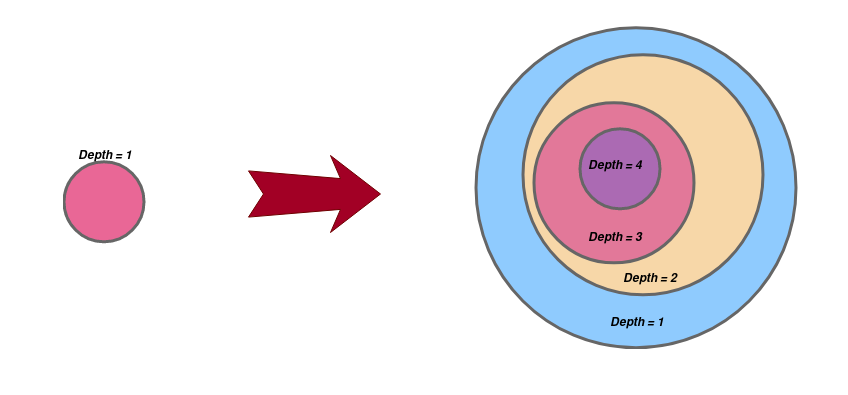
\includegraphics[width=0.9 \linewidth]{figure/livelli}
	\end{center}
	\caption{Esempio di variazione degli attributi di un cluster \label{fig:livelli}}
\end{figure}
Ogni volta che viene creato un oggetto utilizzando una visualizzazione a grafo con modello force directed è necessario un ricalcolo delle forze per ritrovare una posizione di equilibrio che porta ad una visualizzazione gradevole degli oggetti.
Per concludere le primitive di interazione relative alla creazione della visualizzazione di un oggetto del grafo clusterizzato, è di notevole importanza l'ordine con cui queste interazioni vengono eseguite che porta a definire le attenzioni riportate di seguito:
\begin{itemize}
	\item non è possibile creare un arco senza la presenza di due nodi;
	\item non è possibile creare un nodo senza la presenza di un cluster;
	\item non è possibile creare un sotto-cluster senza la presenza di un cluster direttamente collegato alla radice dell'albero di inclusione;
\end{itemize}
\section{Rimozione di un oggetto}
È necessario definire primitive di interazione che portano ad operazioni di oggetti. In questo caso eliminando un oggetto dalla visualizzazione esso verrà eliminato anche dalla struttura dati alla base. Essendo un grafo clusterizzato come visto caratterizzato da tre tipologie di oggetti ognuna di esse avrà delle specifiche caratteristiche. 
Avendo detto poi che ogni elemento del grafo clusterizzato deve avere un interconnessione con ciò che lo circonda, la cancellazione di un oggetto e della sua conseguente visualizzazione porterà a modifiche anche degli elementi ad esso collegati.
La rimozione mediante una interazione di un arco porterà alla cancellazione dell'arco stesso dalla struttura dati e sarà eliminato anche dalla lista degli archi che i nodi, che in precedenza collegava, possiedono.
La rimozione di un nodo causerà:
\begin{itemize}
	\item la rimozione della sua visualizzazione;
	\item la rimozione di tutti gli archi connessi a quel nodo e la loro visualizzazione;
	\item l'eliminazione dalla lista dei nodi del cluster di appartenenza;
	\item nel caso in cui il cluster di appartenenza risultasse vuoto dopo l'eliminazione, dovrà essere eliminato anche suddetto poiché la rappresentazione di un cluster sena nessun oggetto non ha necessità di esistere.
\end{itemize}
Infine la rimozione di un cluster causerà:
\begin{itemize}
	\item la rimozione della sua visualizzazione;
	\item la cancellazione di tutti i nodi appartenenti a quel cluster e di conseguenza di tutti gli archi che intersecavano tali nodi e la loro visualizzazione;
	\item nel caso in cui il cluster direttamente connesso nel cammino dalla radice al cluster eliminato risultasse vuoto dopo l'eliminazione, dovrà essere eliminato anche suddetto;
	\item dovrà essere eseguito un ricalcolo del raggio di tutti i cluster nel cammino dalla radice al cluster cancellato in quanto il raggio è dipendente dal numero di oggetti al suo interno.
\end{itemize}
Ogni qualvolta venga eliminato un oggetto inoltre, nella visualizzazione a grafo con il modello force-directed, si dovranno ricalcolare le forze in gioco per poter trovare nuovamente la posizione di equilibro.

\section{modifica di un oggetto o dell'intero grafo}
Si riportano le operazioni di modifica che possono essere apportate ad un grafo clusterizzato e che saranno analizzate di seguito:
\begin{itemize}
	\item Encode
	\item Riconfigurazione
	\item Spostamento degli oggetti
\end{itemize}
Per quanto concerne lo zooming ed il panning della visualizzazione esse risultano essere uguali a quelle riportate nel capitolo due nella sezione relativa alle primitive di integrazione, in quanto eseguendo queste operazioni in quanto è ininfluente la tipologia di oggetto rappresentato.
\begin{figure}[!htb]
	\begin{center}
		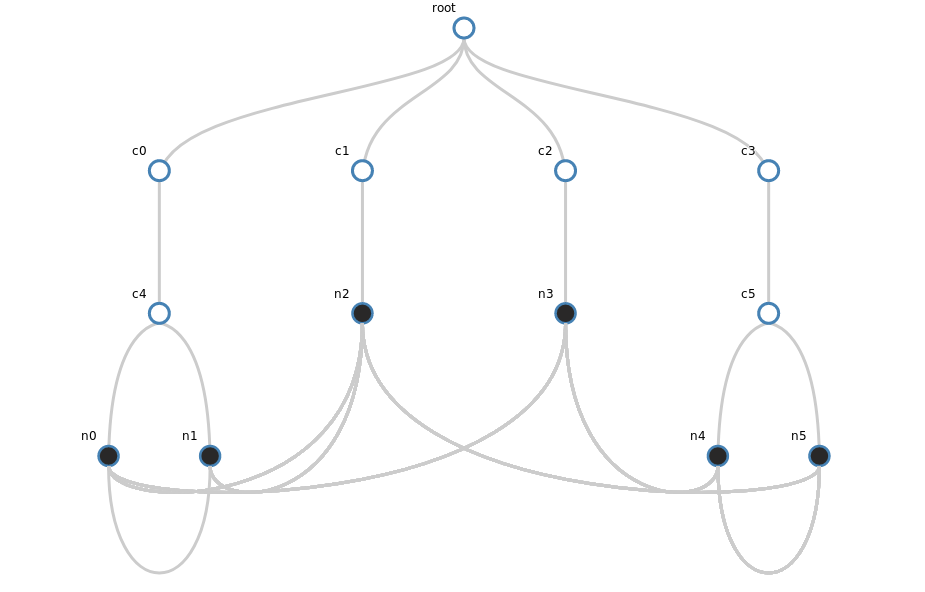
\includegraphics[width=0.9 \linewidth]{figure/grafoAlbero}
	\end{center}
	\caption{esempio di grafo clusterizzato nella visualizzazione ad albero \label{fig:grafoAlbero}}
\end{figure}
\subsection{Encode}
Per quanto concerne l'\textbf{encode} dei dati,essendo un grafo clusterizzato $C$ definito come una coppia $<G,T>$ è possibile eseguire mediante una interazione l'operazione di trasformazione di una visualizzazione. Avendo dei dati è possibile passare da una rappresentazione a grafo ad una ad albero e viceversa avendo cosi diverse possibilità di analisi e tipologie di interazione applicabili. Un esempio della visualizzazione ad albero di un grafo clusterizzato è mostrato nella figura \figurename~\ref{fig:grafoAlbero}.Adottare questo tipo di visualizzazione è molto utile per una visione più chiara della distinzione tra l'albero di inclusione e del grafo sottostante ma la visualizzazione ad albero rende più chiaro il rapporto di inclusione e la distinzione degli archi e dei nodi facendo uso delle coordinate del piano $<x,y>$. Nella visualizzazione ad albero sono inoltre necessarie meno variabili di quelle descritte sopra e riguardanti la visualizzazione a grafo in quanto il raggio degli oggetti è fisso e non è necessario impiegare colori diversi per la distinzione dei vari cluster in quanto è possibile eseguire uno zoom semantico mediante l'utilizzo di etichette che caratterizzano gli elementi del grafo clusterizzato ed in quanto si andrebbe contro il principio per la visualizzazione secondo cui è controproducente utilizzare più variabili di quelle di cui si ha necessità. Inoltre una interfaccia a colori è buona quanto la stessa interfaccia rappresentata in bianco	e nero è ben leggibile. Il colore è dunque necessario solo nel caso in cui si ha bisogno di una codifica aggiuntiva di una variabile, come era nel caso della visualizzazione a grafo per i cluster. Per quanto riguarda i nodi essi possono essere visualizzati con un colore diverso da quello dei cluster.
\subsection{Riconfigurazione}
Mediante la \textbf{riconfigurazione} è possibile riconfigurare una o più caratteristiche associate alla visualizzazione. Utilizzando una rappresentazione a grafo sarà dunque possibile il raggio degli oggetti visualizzati che siano essi nodi o cluster, la palette di colore o aggiungere una descrizione agli oggetti. Si noti che la riconfigurazione può agire sulla visualizzazione dei dati senza modificarne la struttura o cambiare una caratteristica, quale ad esempio il raggio, di cui i dati ne hanno conoscenza. Ogni volta che viene eseguita una riconfigurazione si ha un ridisegno della visualizzazione che spesso porta ad un sostanziale cambiamento della pura rappresentazione avendo così la possibilità di avere molteplici interfacce differenziate per caratteristiche che comunque seguono lo stesso modello scelto e sono collegate agli stessi dati.
\subsection{traslazione}
Per quanto riguarda l'operazione di \textbf{spostamento }degli oggetti, al contrario che nei grafi in cui uno spostamento sul piano della visualizzazione di un nodo deve esclusivamente portare ad uno conseguente di tutti gli archi collegati, nei grafi clusterizzati per lo spostamento di un oggetto è necessario tener conto del mondo circostante avendo quindi due possibili metodi di esecuzione:
\begin{itemize}
	\item impedire la traslazione oltre l'oggetto di appartenenza dando proprietà di solidità ai bordi degli oggetti. Nel caso dei nodi quindi non si potrà traslare oltre il cluster di appartenenza come nel caso del cluster con profondità maggiore di 1 che avrà anche il vincolo dei nodi al suo interno. Questa soluzione limita molto l'interazione in quanto diventa subordinata ai vincoli dati dalla dimensione degli oggetti.
	\item spostare tutti gli elementi collegati a quel nodo in maniera automatica o dovendo eseguire più interazioni. Nel primo caso traslando un oggetto e facendo uso delle connessioni tra i dati si ha la possibilità di muovere tutto ciò che a lui è collegato in una unica interazione. Nel secondo caso risulta essere un processo più lento che porta ad eseguire tante interazioni quanti sono gli oggetti connessi all'oggetto da traslare
\end{itemize}
Ad ogni interazione si dovrà poi ricalcolare il disegno del grafo clusterizzato.Tutte le primitive analizzate danno vita ad uno standard di visualizzazione dei grafi clusterizzati e sono state poi realmente utilizzate per la creazione dell'editor di grafi riportato di seguito per test di analisi delle stesse.
}
